\chapter{内存管理}
在计算机系统(1)中,我们在虚拟存储器部分引出了交换空间的概念。管理内存是硬件和软件协同的结果。
在CPU启动后,内存的地址空间完整提供给第一个启动的软件,也就是操作系统。
随后操作系统在创建每一个进程时分配页表进行页映射,从而提供每个进程完整虚拟地址空间的抽象。
在这个专题的实践中,我们的目标是体验操作系统中不同的内存类型和对应管理内存的方式。

\section{页表和文件页}
目标:读取页表,并且手动修改页表页的映射实现共享(通过\texttt{mmap}调整映射,通过修改内核读取页表);设置文件页实现读写落在文件的指定区域中。具体而言,你需要完成以下两个目标:
\begin{enumerate}
    \item 通过调用mmap对一个virtual memory设定新映射;
    \item 通过调用mmap映射文件后以内存读写的形式访问修改文件(单线程),助教认为你应该需要以下系统调用:open、stat、mmap、munmap,助教认为你可能需要以下系统调用:msync。
\end{enumerate}
\subsection*{指标与评测要求}
文件读写的速度需要能够撑满磁盘带宽。

\subsection*{测试方案}
\begin{enumerate}
    \item \textbf{页表项有效性验证}
    \begin{itemize}
        \item 测试原始的虚拟内存在重新mmap之后物理地址不同。
    \end{itemize}
    
    \item \textbf{内存-文件同步测试}
    \begin{itemize}
        \item 构造3组不同测试文件(空文件/4KB小文件/1MB大数据文件),每种场景测试读后写、跨页写、追加写操作
        \item 通过hexdump工具进行二进制比对验证
    \end{itemize}
\end{enumerate}


\section{内存文件系统}
Linux中提供了内存文件系统(RAMfs)的支持,根据MMU是否使用可以分为有MMU版本和NoMMU版本,分别位于\texttt{fs/ramfs/file-mmu.c}和\texttt{fs/ramfs/file-nommu.c}。
RAMfs无法持久化,在系统崩溃时文件会全部丢失。
现在你需要为RAMfs提供简单的持久化支持,当某个文件被flush到RAMfs时,该文件同步刷到一个预先设置的同步目录中以持久化该文件。
文件系统需要有简单的容错机制,无需保证断电的数据写入,但是必须保证写入的文件原子性操作。(内容可以不完整,但是不能出现orphan inode)
目标:增加flush下的文件持久化。

接口设计补充:你可以使用FUSE在用户态支持,也可以在内核态增加接口。一个可能的接口样式如下:
\begin{lstlisting}[language=C]
int ramfs_bind(char *sync_dir);             // 绑定后端写入的文件
int ramfs_file_flush(struct file *file);    // 同步触发接口
\end{lstlisting}


\subsection*{测试方案}
\begin{enumerate}
    \item \textbf{单文件持久化正确性}
    \begin{itemize}
        \item 构造读写请求在以下时机触发flush:立即写入、页缓存(Page Cache)满时写入、定时器触发写入,要求不崩溃
        \item 验证文件内容和写入的一致性
    \end{itemize}
    
    \item \textbf{多线程顺序一致性}
    \begin{itemize}
        \item 创建10个生产者线程进行高频写操作(含时间戳标记),创建3个消费者线程随机触发flush。验证最终持久化文件中的操作顺序满足Lamport happens-before关系。
        \item 交错执行append和truncate操作的临界情况
    \end{itemize}
    
    \item \textbf{异常场景测试}
    \begin{itemize}
        \item 在flush过程中注入断电模拟(通过sysrq触发kernel panic),恢复后验证文件系统的完整性约束
    \end{itemize}
\end{enumerate}



\section{内存压力导向的内存管理}
MacOS给出内存压力的概念,相比于UNIX的swap大小,它被认为是更好的表达虚拟内存健康程度的标志。

\begin{figure}[h]
    \centering
    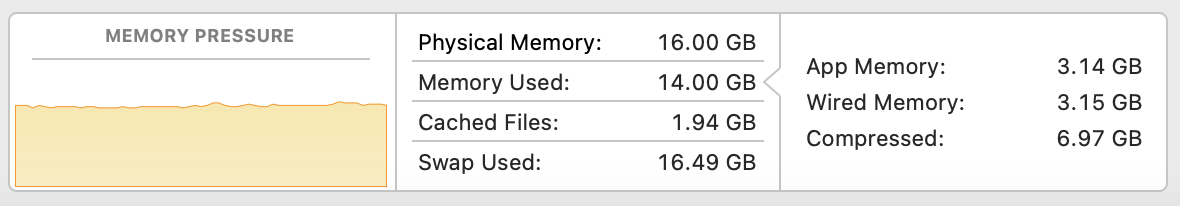
\includegraphics[width=0.8\linewidth]{figure/mixed-figures/memory-pressure.png}
    \caption{MacOS中的内存压力}
    \label{fig:enter-label}
\end{figure}

目标:该实践任务包含两个子任务点。
\begin{enumerate}
    \item 利用Linux的Wired Memory(即Active Memory)和压缩内存给出一个Linux下的内核内存压力指示器。
    \item 在用户态划出一块内存空间,实现一个简单的基于内存压力的交换策略。
\end{enumerate}


提示:区分wired memory和inactive memory的区别。

测试:测试内存压力和感知准确度的对比(演示),测试交换策略。
